
\فصل{آزمون حافظه}



\قسمت{آشنایی با آزمون حافظه}

آزمون حافظه به فرآیند تست کردن تایید کارکرد، درستی و کارایی حافظه سیستم گفته می‌شود. در این جا ما در فایل اصلی پروژه یعنی \لر{MemTest.c} ۴ نوع تست آماده کرده‌ایم که هر کدام برای شرایطی خاص مناسب هستند.

\قسمت{آزمون‌ها}

\زیرقسمت{\لر{Walking Ones}}

در این آزمون ما با یک الگو که شامل دقیقا یک بیت ۱ است شروع می‌کنیم و هر بار مقدار آن را یک شیفت دوری می‌دهیم. سپس در نهایت همه مقادیر را چک می‌کنیم. این آزمون کمک می‌کند مشکلات \لر{data bus} پیدا شود. دلیل ۱ بودن دقیقا یک بیت این است که تفاوت یک بیت با دو بیت کناری شانس خطا را افزایش می‌دهد. این تست در تابع \لر{WalkingOnesTest} پیاده‌سازی شده است.

\زیرقسمت{\لر{Identity}}

در این آزمون ما در هر خانه از حافظه آدرس خودش را می‌نویسیم. سپس در نهایت همه مقادیر را چک می‌کنیم. این آزمون بسیار ساده و کلی است و. در تابع \لر{IdentityTest} پیاده‌سازی شده است.

\زیرقسمت{\لر{Rowhammer}}

در این آزمون ما حساس بودن حافظه به آسیب پذیری \لر{Rowhammer} را می‌سنجیم. این آسیب پذیری سعی می‌کند با دسترسی با فرکانس بالا به چند سطر خاص در حافظه باعث شود مقادیر سطری دیگر عوض شوند. در این جا ما با استناد به \href{https://github.com/google/rowhammer-test/blob/master/double_sided_rowhammer.cc}{این} پیاده‌سازی از \لر{Rowhammer} دو طرفه، تابع \لر{RowHammerTest} را پیاده‌سازی کرده‌ایم.

\زیرقسمت{\لر{DMA}}

در این آزمون ما درستی کارکرد زیرسامانه \لر{DMA} برای انتقال داده بین دیسک و حافظه بدون دخالت پردازنده را می‌سنجیم. برای این کار در ابتدا یک فایل روی دیسک مورد نظر ساخته و با داده‌های خاص پر می‌شود. سپس این فایل در خانه‌هایی از حافظه خوانده شده و چک می‌شود که با چیزی که نوشته شده یکی باشد. این تست در تابع \لر{DMA} پیاده‌سازی شده است.

\قسمت{اجرای آزمون حافظه}

در \رجوع{fig:test1} یک اجرا از تست‌های نوشته شده را نشان می‌دهیم.
\begin{figure}
	\centering
	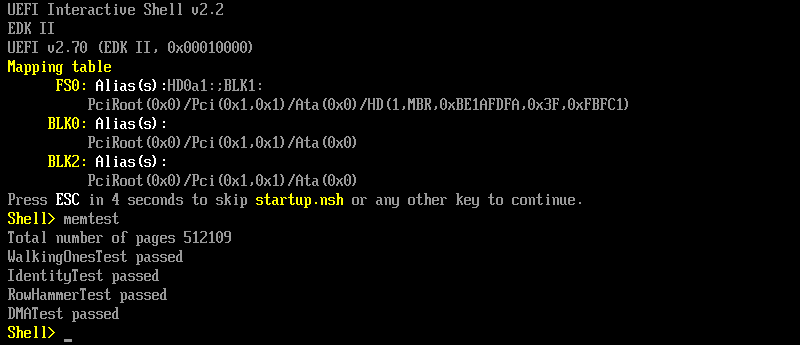
\includegraphics[width=0.7\linewidth]{figs/test/test1}
	\caption{اجرای متوالی همه‌ی آزمون‌ها}
	\label{fig:test1}
\end{figure}


